\documentclass{article}
\usepackage[margin=2cm]{geometry}
\usepackage[utf8]{inputenc}
\usepackage{minted}
\usepackage{amsfonts}
\usepackage{amsmath}
\usepackage{tikz}

\title{CSC258 PRELAB 6}
\author{Tingfeng Xia}
\date{October 2019}

\usepackage{natbib}
\usepackage{graphicx}

\begin{document}

\maketitle
\section*{PART I}
\paragraph{2.} The \texttt{reset\_n} signal is synchronus and active low, meaning it will trigger at a clock $1\rightarrow 0$ if the reset is at logic low. In order to reset, I should set \texttt{reset\_n}$\gets 0$ and hold until the following clock negedge, allowing set-up and hold-stable time.
\paragraph{3.} Here is my code for the FSM. It was extended based on the given starter code in the lab handout:
\begin{minted}{verilog}
    // (*) Note: Using starter code provided on Quercus
    // SW[0]: reset signal
    // SW[1]: input signal (w)

    // KEY[0]: clock

    // LEDR[2:0]: current state
    // LEDR[9]: output (z)

    // SW[0]:       reset signal
    // SW[1]:       input signal (w)

    // KEY[0]:      clock

    // LEDR[2:0]:   current state
    // LEDR[9]:     output (z)

    module sequence_detector(SW, KEY, LEDR);
        input [9:0] SW;
        input [3:0] KEY;
        output [9:0] LEDR;

        wire w, clock, resetn, z;
        
        reg [2:0] y_Q, Y_D; // y_Q represents current state, Y_D represents next state
    
        // (*) Note: Here our local param is for specification purpose of the states!
        localparam A = 3'b000, B = 3'b001, C = 3'b010, D = 3'b011, E = 3'b100, F = 3'b101, G = 3'b110;
        
        // Connect inputs and outputs to internal wires
        assign w = SW[1];
        assign clock = ~KEY[0];
        assign resetn = SW[0];
        assign LEDR[9] = z;
        assign LEDR[2:0] = y_Q;

        // State table
        // The state table should only contain the logic for state transitions
        // Do not mix in any output logic.  The output logic should be handled separately.
        // This will make it easier to read, modify and debug the code.
        always @(*)
        begin   // Start of state_table
            case (y_Q)
                A: begin
                    if (!w) Y_D = A;
                    else Y_D = B;
                    end
                B: begin
                    if (!w) Y_D = A;
                    else Y_D = C;
                    end
                C: begin
                        if (!w) Y_D = E;
                        else Y_D = D;
                    end
                D: begin
                        if (!w) Y_D = E;
                        else Y_D = F;
                    end
                E: begin
                        if (!w) Y_D = A;
                        else Y_D = G;
                    end
                F: begin
                        if (!w) Y_D = E;
                        else Y_D = F;
                    end
                G: begin
                        if (!w) Y_D = A;
                        else Y_D = C;
                    end
                default: Y_D = A;
            endcase
        end     
        // End of state_table

        // State Register (i.e., FFs)
        always @(posedge clock)
        begin   // Start of state_FFs (state register)
            if(resetn == 1'b0)
                y_Q <= A;
            else
                y_Q <= Y_D;
        end     // End of state_FFs (state register)

        // Output logic
        // Set z to 1 to turn on LED when in relevant states
        assign z = ((y_Q == F) || (y_Q == G));  
    endmodule
\end{minted}
\paragraph{4.} Here is my modelsim results. Notice that the states are incrementing. 
\begin{center}
    \includegraphics[scale=0.19]{q1_modelsim.png}
\end{center}

\section*{PART II}
\paragraph{3.} Here is FSM state diagram:
\begin{small}
    \begin{center}
        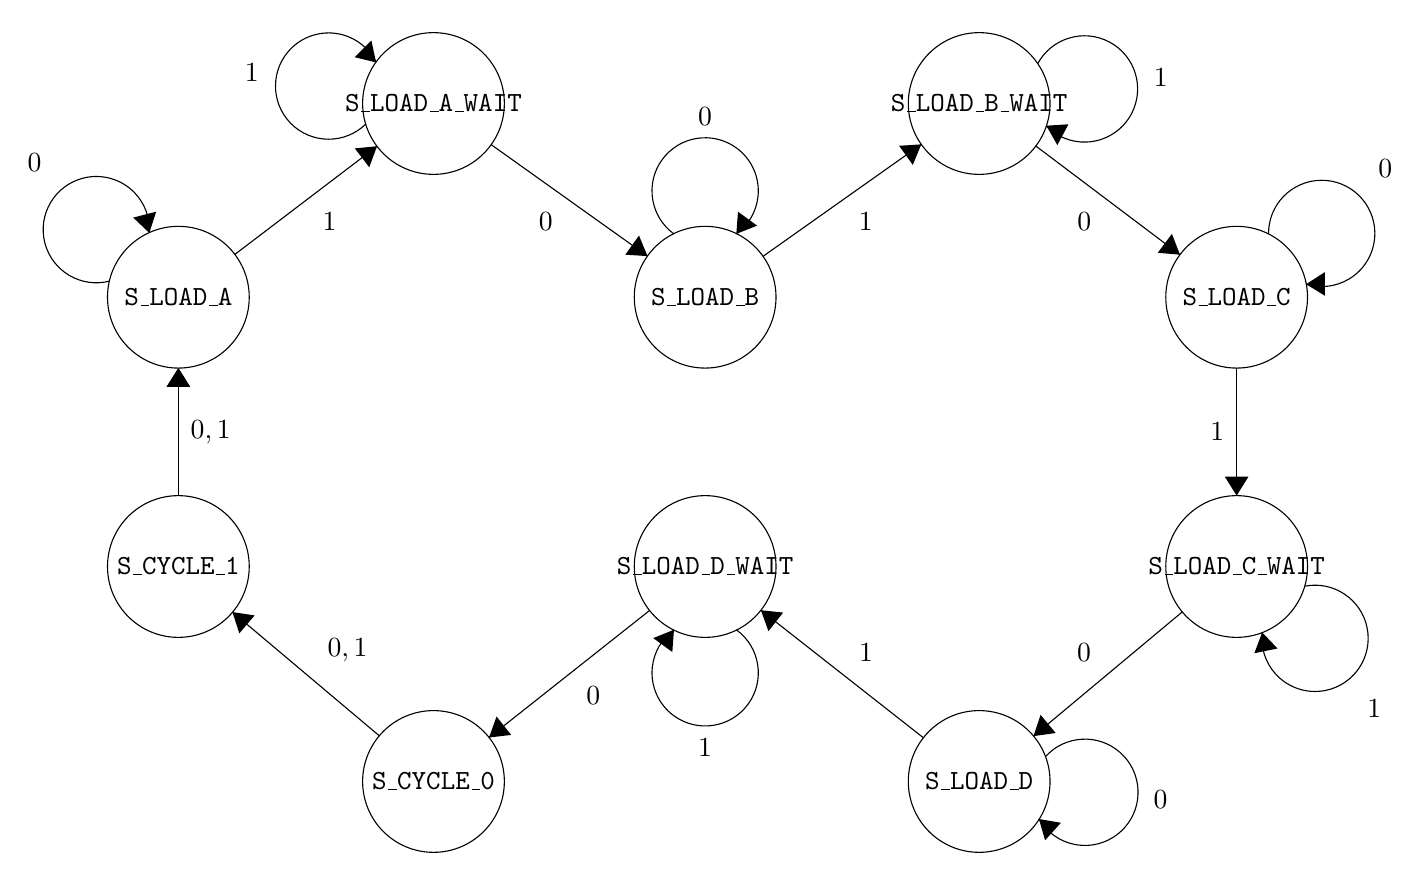
\begin{tikzpicture}[scale=0.3]
            \tikzstyle{every node}+=[inner sep=0pt]
            \draw [black] (14.2,-17.2) circle (3);
            \draw (14.2,-17.2) node {\texttt{S\_LOAD\_A}};
            \draw [black] (25,-9) circle (3);
            \draw (25,-9) node {\texttt{S\_LOAD\_A\_WAIT}};
            \draw [black] (36.5,-17.2) circle (3);
            \draw (36.5,-17.2) node {\texttt{S\_LOAD\_B}};
            \draw [black] (48.1,-9) circle (3);
            \draw (48.1,-9) node {\texttt{S\_LOAD\_B\_WAIT}};
            \draw [black] (59,-17.2) circle (3);
            \draw (59,-17.2) node {\texttt{S\_LOAD\_C}};
            \draw [black] (59,-28.6) circle (3);
            \draw (59,-28.6) node {\texttt{S\_LOAD\_C\_WAIT}};
            \draw [black] (48.1,-37.7) circle (3);
            \draw (48.1,-37.7) node {\texttt{S\_LOAD\_D}};
            \draw [black] (36.5,-28.6) circle (3);
            \draw (36.5,-28.6) node {\texttt{S\_LOAD\_D\_WAIT}};
            \draw [black] (25,-37.7) circle (3);
            \draw (25,-37.7) node {\texttt{S\_CYCLE\_0}};
            \draw [black] (14.2,-28.6) circle (3);
            \draw (14.2,-28.6) node {\texttt{S\_CYCLE\_1}};
            \draw [black] (16.59,-15.39) -- (22.61,-10.81);
            \fill [black] (22.61,-10.81) -- (21.67,-10.9) -- (22.28,-11.7);
            \draw (20.6,-13.6) node [below] {$1$};
            \draw [black] (27.44,-10.74) -- (34.06,-15.46);
            \fill [black] (34.06,-15.46) -- (33.7,-14.59) -- (33.12,-15.4);
            \draw (29.75,-13.6) node [below] {$0$};
            \draw [black] (38.95,-15.47) -- (45.65,-10.73);
            \fill [black] (45.65,-10.73) -- (44.71,-10.79) -- (45.29,-11.6);
            \draw (43.3,-13.6) node [below] {$1$};
            \draw [black] (50.5,-10.8) -- (56.6,-15.4);
            \fill [black] (56.6,-15.4) -- (56.26,-14.52) -- (55.66,-15.32);
            \draw (52.55,-13.6) node [below] {$0$};
            \draw [black] (59,-20.2) -- (59,-25.6);
            \fill [black] (59,-25.6) -- (59.5,-24.8) -- (58.5,-24.8);
            \draw (58.5,-22.9) node [left] {$1$};
            \draw [black] (56.7,-30.52) -- (50.4,-35.78);
            \fill [black] (50.4,-35.78) -- (51.34,-35.65) -- (50.7,-34.88);
            \draw (52.54,-32.66) node [above] {$0$};
            \draw [black] (45.74,-35.85) -- (38.86,-30.45);
            \fill [black] (38.86,-30.45) -- (39.18,-31.34) -- (39.8,-30.55);
            \draw (43.31,-32.65) node [above] {$1$};
            \draw [black] (34.15,-30.46) -- (27.35,-35.84);
            \fill [black] (27.35,-35.84) -- (28.29,-35.73) -- (27.67,-34.95);
            \draw (31.76,-33.65) node [below] {$0$};
            \draw [black] (22.71,-35.77) -- (16.49,-30.53);
            \fill [black] (16.49,-30.53) -- (16.78,-31.43) -- (17.43,-30.67);
            \draw (21.36,-32.66) node [above] {$0,1$};
            \draw [black] (14.2,-25.6) -- (14.2,-20.2);
            \fill [black] (14.2,-20.2) -- (13.7,-21) -- (14.7,-21);
            \draw (14.7,-22.9) node [right] {$0,1$};
            \draw [black] (11.291,-16.517) arc (284.52754:-3.47246:2.25);
            \draw (8.43,-11.48) node [left] {$0$};
            \fill [black] (12.97,-14.48) -- (13.26,-13.58) -- (12.29,-13.83);
            \draw [black] (22.14,-9.865) arc (314.55884:26.55884:2.25);
            \draw (17.63,-7.67) node [left] {$1$};
            \fill [black] (22.57,-7.26) -- (22.37,-6.33) -- (21.66,-7.04);
            \draw [black] (35.177,-14.52) arc (234:-54:2.25);
            \draw (36.5,-9.95) node [above] {$0$};
            \fill [black] (37.82,-14.52) -- (38.7,-14.17) -- (37.89,-13.58);
            \draw [black] (37.823,-31.28) arc (54:-234:2.25);
            \draw (36.5,-35.85) node [below] {$1$};
            \fill [black] (35.18,-31.28) -- (34.3,-31.63) -- (35.11,-32.22);
            \draw [black] (50.573,-7.323) arc (151.87806:-136.12194:2.25);
            \draw (55.47,-7.91) node [right] {$1$};
            \fill [black] (50.94,-9.94) -- (51.41,-10.76) -- (51.88,-9.88);
            \draw [black] (60.35,-14.534) arc (180.8699:-107.1301:2.25);
            \draw (64.98,-11.75) node [right] {$0$};
            \fill [black] (61.94,-16.65) -- (62.74,-17.14) -- (62.73,-16.14);
            \draw [black] (61.869,-29.436) arc (101.48955:-186.51045:2.25);
            \draw (64.51,-34.62) node [right] {$1$};
            \fill [black] (60.08,-31.39) -- (59.75,-32.27) -- (60.73,-32.07);
            \draw [black] (50.9,-36.657) arc (138.16468:-149.83532:2.25);
            \draw (55.46,-38.48) node [right] {$0$};
            \fill [black] (50.63,-39.29) -- (50.89,-40.19) -- (51.56,-39.45);
            \draw [black] (14.2,-25.6) -- (14.2,-20.2);
            \fill [black] (14.2,-20.2) -- (13.7,-21) -- (14.7,-21);
        \end{tikzpicture}
        \end{center}
\end{small}

\paragraph{4.} Here is my modified code
\begin{minted}{verilog}
    //Sw[7:0] data_in
    //KEY[0] synchronous reset when pressed
    //KEY[1] go signal

    //LEDR displays result
    //HEX0 & HEX1 also displays result

    module poly_function(SW, KEY, CLOCK_50, LEDR, HEX0, HEX1);
        input [9:0] SW;
        input [3:0] KEY;
        input CLOCK_50;
        output [9:0] LEDR;
        output [6:0] HEX0, HEX1;

        wire resetn;
        wire go;

        wire [7:0] data_result;
        assign go = ~KEY[1];
        assign resetn = KEY[0];

        part2 u0(
            .clk(CLOCK_50),
            .resetn(resetn),
            .go(go),
            .data_in(SW[7:0]),
            .data_result(data_result)
        );
        
        assign LEDR[9:0] = {2'b00, data_result};

        hex_decoder H0(
            .hex_digit(data_result[3:0]), 
            .segments(HEX0)
        );
            
        hex_decoder H1(
            .hex_digit(data_result[7:4]), 
            .segments(HEX1)
        );

    endmodule

    module part2(
            input clk,
            input resetn,
            input go,
            input [7:0] data_in,
            output [7:0] data_result
        );

        // lots of wires to connect our datapath and control
        wire ld_a, ld_b, ld_c, ld_x, ld_r;
        wire ld_alu_out;
        wire [1:0]  alu_select_a, alu_select_b;
        wire alu_op;

        control C0(
            .clk(clk),
            .resetn(resetn),
            
            .go(go),
            
            .ld_alu_out(ld_alu_out), 
            .ld_x(ld_x),
            .ld_a(ld_a),
            .ld_b(ld_b),
            .ld_c(ld_c), 
            .ld_r(ld_r), 
            
            .alu_select_a(alu_select_a),
            .alu_select_b(alu_select_b),
            .alu_op(alu_op)
        );

        datapath D0(
            .clk(clk),
            .resetn(resetn),

            .ld_alu_out(ld_alu_out), 
            .ld_x(ld_x),
            .ld_a(ld_a),
            .ld_b(ld_b),
            .ld_c(ld_c), 
            .ld_r(ld_r), 

            .alu_select_a(alu_select_a),
            .alu_select_b(alu_select_b),
            .alu_op(alu_op),

            .data_in(data_in),
            .data_result(data_result)
        );
                    
    endmodule        
                    

    module control(
            input clk,
            input resetn,
            input go,

            output reg  ld_a, ld_b, ld_c, ld_x, ld_r,
            output reg  ld_alu_out,
            output reg [1:0]  alu_select_a, alu_select_b,
            output reg alu_op
        );

        reg [3:0] current_state, next_state; 
        
        localparam  S_LOAD_A        = 4'd0,
                    S_LOAD_A_WAIT   = 4'd1,
                    S_LOAD_B        = 4'd2,
                    S_LOAD_B_WAIT   = 4'd3,
                    S_LOAD_C        = 4'd4,
                    S_LOAD_C_WAIT   = 4'd5,
                    S_LOAD_X        = 4'd6,
                    S_LOAD_X_WAIT   = 4'd7,
                    S_CYCLE_0       = 4'd8,
                    S_CYCLE_1       = 4'd9,
                    S_CYCLE_2       = 4'd10,
                    S_CYCLE_3       = 4'd11,
                    S_CYCLE_4       = 4'd12;
        
        // Next state logic aka our state table
        always@(*)
        begin: state_table 
                case (current_state)
                    // Loop in current state until value is input
                    S_LOAD_A: next_state = go ? S_LOAD_A_WAIT : S_LOAD_A; 
                    // Loop in current state until go signal goes low
                    S_LOAD_A_WAIT: next_state = go ? S_LOAD_A_WAIT : S_LOAD_B; 
                    // Loop in current state until value is input
                    S_LOAD_B: next_state = go ? S_LOAD_B_WAIT : S_LOAD_B; 
                    // Loop in current state until go signal goes low
                    S_LOAD_B_WAIT: next_state = go ? S_LOAD_B_WAIT : S_LOAD_C; 
                    // Loop in current state until value is input
                    S_LOAD_C: next_state = go ? S_LOAD_C_WAIT : S_LOAD_C; 
                    // Loop in current state until go signal goes low
                    S_LOAD_C_WAIT: next_state = go ? S_LOAD_C_WAIT : S_LOAD_X; 
                    // Loop in current state until value is input
                    S_LOAD_X: next_state = go ? S_LOAD_X_WAIT : S_LOAD_X; 
                    // Loop in current state until go signal goes low
                    S_LOAD_X_WAIT: next_state = go ? S_LOAD_X_WAIT : S_CYCLE_0; 
                    S_CYCLE_0: next_state = S_CYCLE_1;
                    // we will be done our two operations, start over after
                    S_CYCLE_1: next_state = S_CYCLE_2;
                    S_CYCLE_2: next_state = S_CYCLE_3;
                    S_CYCLE_3: next_state = S_CYCLE_4;
                    S_CYCLE_4: next_state = S_LOAD_A; 
                default:     next_state = S_LOAD_A;
            endcase
        end // state_table
    

        // Output logic aka all of our datapath control signals
        always @(*)
        begin: enable_signals
            // By default make all our signals 0
            ld_alu_out = 1'b0;
            ld_a = 1'b0;
            ld_b = 1'b0;
            ld_c = 1'b0;
            ld_x = 1'b0;
            ld_r = 1'b0;
            alu_select_a = 2'b00;
            alu_select_b = 2'b00;
            alu_op       = 1'b0;

            case (current_state)
                S_LOAD_A: begin
                    ld_a = 1'b1;
                    end
                S_LOAD_B: begin
                    ld_b = 1'b1;
                    end
                S_LOAD_C: begin
                    ld_c = 1'b1;
                    end
                S_LOAD_X: begin
                    ld_x = 1'b1;
                    end
                S_CYCLE_0:
                    begin
                    ld_alu_out = 1'b1;
                        ld_a = 1'b1;
                        alu_select_a = 2'b00;
                        alu_select_b = 2'b11;
                        alu_op = 1'b1;
                end
                S_CYCLE_1: 
                    begin
                        ld_alu_out = 1'b1;
                        ld_a = 1'b1;
                        alu_select_a = 2'b00;
                        alu_select_b = 2'b11;
                        alu_op = 1'b1;
                end
                    S_CYCLE_2: 
                    begin
                        ld_alu_out = 1'b1;
                        ld_b = 1'b1;
                        alu_select_a = 2'b01;
                        alu_select_b = 2'b11;
                        alu_op = 1'b1;
                end
                    S_CYCLE_3: 
                    begin
                        ld_alu_out = 1'b1;
                        ld_a = 1'b1;
                        alu_select_a = 2'b00;
                        alu_select_b = 2'b01;
                        alu_op = 1'b0;
                end
                    S_CYCLE_4: 
                    begin
                        ld_r = 1'b1;
                        alu_select_a = 2'b00;
                        alu_select_b = 2'b10;
                        alu_op = 1'b0;
                end
            // default:    // don't need default since we already made sure all of our outputs were assigned a value at the start of the always block
            endcase
        end // enable_signals
    
        // current_state registers
        always@(posedge clk)
        begin: state_FFs
            if(!resetn)
                current_state <= S_LOAD_A;
            else
                current_state <= next_state;
        end // state_FFS
    endmodule

    // (*) Note: Specifying the I/O in the function header is also possible.
    module datapath(
            input clk,
            input resetn,
            input [7:0] data_in,
            input ld_alu_out, 
            input ld_x, ld_a, ld_b, ld_c,
            input ld_r,
            input alu_op, 
            input [1:0] alu_select_a, alu_select_b,
            output reg [7:0] data_result
        );
        
        // input registers
        reg [7:0] a, b, c, x;

        // output of the alu
        reg [7:0] alu_out;
        // alu input muxes
        reg [7:0] alu_a, alu_b;
        
        // Registers a, b, c, x with respective input logic
        always @ (posedge clk) begin
            if (!resetn) begin
                a <= 8'd0; 
                b <= 8'd0; 
                c <= 8'd0; 
                x <= 8'd0; 
            end
            else begin
                if (ld_a)
                    a <= ld_alu_out ? alu_out : data_in; 
                    // load alu_out if load_alu_out signal is high, otherwise load from data_in
                if (ld_b)
                    b <= ld_alu_out ? alu_out : data_in; 
                    // load alu_out if load_alu_out signal is high, otherwise load from data_in
                if (ld_x)
                    x <= data_in;

                if (ld_c)
                    c <= data_in;
            end
        end
    
        // Output result register
        always @ (posedge clk) begin
            if (!resetn) begin
                data_result <= 8'd0; 
            end
            else 
                if(ld_r)
                    data_result <= alu_out;
        end

        // The ALU input multiplexers
        always @(*)
        begin
            case (alu_select_a)
                2'd0:
                    alu_a = a;
                2'd1:
                    alu_a = b;
                2'd2:
                    alu_a = c;
                2'd3:
                    alu_a = x;
                default: alu_a = 8'd0;
            endcase

            case (alu_select_b)
                2'd0:
                    alu_b = a;
                2'd1:
                    alu_b = b;
                2'd2:
                    alu_b = c;
                2'd3:
                    alu_b = x;
                default: alu_b = 8'd0;
            endcase
        end

        // The ALU 
        always @(*)
        begin : ALU
            // alu
            case (alu_op)
                0: begin
                    alu_out = alu_a + alu_b; //performs addition
                end
                1: begin
                    alu_out = alu_a * alu_b; //performs multiplication
                end
                default: alu_out = 8'd0;
            endcase
        end
        
    endmodule

    // re-written using hexadecimal, this is better!
    // New implementation in the handout
    module hex_decoder(hex_digit, segments);
        input [3:0] hex_digit;
        output reg [6:0] segments;
    
        always @(*)
            case (hex_digit)
                4'h0: segments = 7'b100_0000;
                4'h1: segments = 7'b111_1001;
                4'h2: segments = 7'b010_0100;
                4'h3: segments = 7'b011_0000;
                4'h4: segments = 7'b001_1001;
                4'h5: segments = 7'b001_0010;
                4'h6: segments = 7'b000_0010;
                4'h7: segments = 7'b111_1000;
                4'h8: segments = 7'b000_0000;
                4'h9: segments = 7'b001_1000;
                4'hA: segments = 7'b000_1000;
                4'hB: segments = 7'b000_0011;
                4'hC: segments = 7'b100_0110;
                4'hD: segments = 7'b010_0001;
                4'hE: segments = 7'b000_0110;
                4'hF: segments = 7'b000_1110;   
                default: segments = 7'h7f;
            endcase
    endmodule

\end{minted}

\paragraph{5.} FSM produced by Quartus, see the screen shot
\begin{center}
    \includegraphics[scale=0.19]{quartus_fsm.png}
    \includegraphics[scale=0.19]{quartus_statetable.png}
\end{center}
\paragraph{6.} ModelSim results, see the below screen shot
\begin{center}
    \includegraphics[scale=0.19]{q2_sim.png}
\end{center}

\begin{Large}
    Above is simulations that I did when testing modules, but it is rather hard to demonstrate how the module works. I did a simple example below. \newline \newline
\end{Large}

I will demonstrate this using 
\begin{align*}
    A &\gets 7_{10} \equiv 00001111_2 \\
    B &\gets 5_{10} \equiv 00000101_2 \\
    C &\gets 3_{10} \equiv 00000011_2 \\
    x &\gets 1_{10} \equiv 00000001_2
\end{align*}
Then, the expected result is
\begin{equation*}
    Cx^2 + Bx + A = 15_{10} \equiv 00001111_2
\end{equation*}
Indeed, we have
\begin{center}
    \includegraphics[scale=0.19]{q2_simple_demo.png}
\end{center}

\end{document}
